
\let\negmedspace\undefined
\let\negthickspace\undefined
\documentclass[journal,12pt,twocolumn]{IEEEtran}
%\documentclass[conference]{IEEEtran}
%\IEEEoverridecommandlockouts
% The preceding line is only needed to identify funding in the first footnote. If that is unneeded, please comment it out.
\usepackage{svg}
\usepackage{tikz, pgfplots}
\usepackage{cite}
\usepackage{amsmath,amssymb,amsfonts,amsthm}
\usepackage{algorithmic}
\usepackage{graphicx,wrapfig}
\usepackage{textcomp}
\usepackage{xcolor}
\usepackage{txfonts}
\usepackage{listings}
\usepackage{enumitem}
\usepackage{mathtools}
\usepackage{gensymb}
\usepackage[breaklinks=true]{hyperref}
\usepackage{tkz-euclide} % loads  TikZ and tkz-base
\usepackage{listings}
\usetikzlibrary{positioning}
%
%\usepackage{setspace}
%\usepackage{gensymb}
%\doublespacing
%\singlespacing

%\usepackage{graphicx}
%\usepackage{amssymb}
%\usepackage{relsize}
%\usepackage[cmex10]{amsmath}
%\usepackage{amsthm}
%\interdisplaylinepenalty=2500
%\savesymbol{iint}
%\usepackage{txfonts}
%\restoresymbol{TXF}{iint}
%\usepackage{wasysym}
%\usepackage{amsthm}
%\usepackage{iithtlc}
%\usepackage{mathrsfs}
%\usepackage{txfonts}
%\usepackage{stfloats}
%\usepackage{bm}
%\usepackage{cite}
%\usepackage{cases}
%\usepackage{subfig}
%\usepackage{xtab}
%\usepackage{longtable}
%\usepackage{multirow}
%\usepackage{algorithm}
%\usepackage{algpseudocode}
%\usepackage{enumitem}
%\usepackage{mathtools}
%\usepackage{tikz}
%\usepackage{circuitikz}
%\usepackage{verbatim}
%\usepackage{tfrupee}
%\usepackage{stmaryrd}
%\usetkzobj{all}
%    \usepackage{color}                                            %%
%    \usepackage{array}                                            %%
%    \usepackage{longtable}                                        %%
%    \usepackage{calc}                                             %%
%    \usepackage{multirow}                                         %%
%    \usepackage{hhline}                                           %%
%    \usepackage{ifthen}                                           %%
  %optionally (for landscape tables embedded in another document): %%
%    \usepackage{lscape}     
%\usepackage{multicol}
%\usepackage{chngcntr}
%\usepackage{enumerate}

%\usepackage{wasysym}
%\newcounter{MYtempeqncnt}
\DeclareMathOperator*{\Res}{Res}
%\renewcommand{\baselinestretch}{2}
\renewcommand\thesection{\arabic{section}}
\renewcommand\thesubsection{\thesection.\arabic{subsection}}
\renewcommand\thesubsubsection{\thesubsection.\arabic{subsubsection}}

\renewcommand\thesectiondis{\arabic{section}}
\renewcommand\thesubsectiondis{\thesectiondis.\arabic{subsection}}
\renewcommand\thesubsubsectiondis{\thesubsectiondis.\arabic{subsubsection}}

% correct bad hyphenation here
\hyphenation{op-tical net-works semi-conduc-tor}
\def\inputGnumericTable{}                                 %%

\lstset{
%language=C,
frame=single, 
breaklines=true,
columns=fullflexible
}
%\lstset{
%language=tex,
%frame=single, 
%breaklines=true
%}

\begin{document}
%


\newtheorem{theorem}{Theorem}[section]
\newtheorem{problem}{Problem}
\newtheorem{proposition}{Proposition}[section]
\newtheorem{lemma}{Lemma}[section]
\newtheorem{corollary}[theorem]{Corollary}
\newtheorem{example}{Example}[section]
\newtheorem{definition}[problem]{Definition}
%\newtheorem{thm}{Theorem}[section] 
%\newtheorem{defn}[thm]{Definition}
%\newtheorem{algorithm}{Algorithm}[section]
%\newtheorem{cor}{Corollary}
\newcommand{\BEQA}{\begin{eqnarray}}
		\newcommand{\EEQA}{\end{eqnarray}}
\newcommand{\define}{\stackrel{\triangle}{=}}

\bibliographystyle{IEEEtran}
%\bibliographystyle{ieeetr}


\providecommand{\mbf}{\mathbf}
\providecommand{\pr}[1]{\ensuremath{\Pr\left(#1\right)}}
\providecommand{\qfunc}[1]{\ensuremath{Q\left(#1\right)}}
\providecommand{\sbrak}[1]{\ensuremath{{}\left[#1\right]}}
\providecommand{\lsbrak}[1]{\ensuremath{{}\left[#1\right.}}
\providecommand{\rsbrak}[1]{\ensuremath{{}\left.#1\right]}}
\providecommand{\brak}[1]{\ensuremath{\left(#1\right)}}
\providecommand{\lbrak}[1]{\ensuremath{\left(#1\right.}}
\providecommand{\rbrak}[1]{\ensuremath{\left.#1\right)}}
\providecommand{\cbrak}[1]{\ensuremath{\left\{#1\right\}}}
\providecommand{\lcbrak}[1]{\ensuremath{\left\{#1\right.}}
\providecommand{\rcbrak}[1]{\ensuremath{\left.#1\right\}}}
\theoremstyle{remark}
\newtheorem{rem}{Remark}
\newcommand{\sgn}{\mathop{\mathrm{sgn}}}
\providecommand{\abs}[1]{\(left\)vert#1\(right\)vert}
\providecommand{\res}[1]{\Res\displaylimits_{#1}}
\providecommand{\norm}[1]{\(left\)lVert#1\(right\)rVert}
%\providecommand{\norm}[1]{\lVert#1\rVert}
\providecommand{\mtx}[1]{\mathbf{#1}}
\providecommand{\mean}[1]{E\(left\)[ #1 \(right\)]}
\providecommand{\fourier}{\overset{\mathcal{F}}{ \rightleftharpoons}}
%\providecommand{\hilbert}{\overset{\mathcal{H}}{ \rightleftharpoons}}
\providecommand{\system}{\overset{\mathcal{H}}{ \longleftrightarrow}}
%\newcommand{\solution}[2]{\textbf{Solution:}{#1}}
\newcommand{\solution}{\noindent \textbf{Solution: }}
\newcommand{\cosec}{\,\text{cosec}\,}
\providecommand{\dec}[2]{\ensuremath{\overset{#1}{\underset{#2}{\gtrless}}}}
\newcommand{\myvec}[1]{\ensuremath{\begin{pmatrix}#1\end{pmatrix}}}
\newcommand{\mydet}[1]{\ensuremath{\begin{vmatrix}#1\end{vmatrix}}}

\let\vec\mathbf


\vspace{3cm}

\title{
	%	\logo{
	Assignment:- 2
 
	\Large AI1110: Probability and Random Variables
 
	\Large Indian Institute of Technology, Hyderabad
	%	}
}
\author{
	CS22BTECH11001
	
	Aayush Adlakha
 
	29 April, 2023
	% <-this % stops a space
}






\maketitle

\newpage


\bigskip
\renewcommand{\thefigure}{\theenumi}
\renewcommand{\thetable}{\theenumi}
\textbf{Exemplar 11.16.3.11}
The accompanying Venn diagram shows three events, A, B, and C, and also the probabilities of the various intersections (for instance, \pr{AB} = .07). Determine
\begin{enumerate}[label=(\alph*)]
\item 
\pr{A}
\item 
\pr{BC^\prime}
\item 
\pr{A + B}
\item 
\pr{AB^\prime}
\item 
\pr{BC}
\item 
Probability of exactly one
of the three occurs.
\end{enumerate}
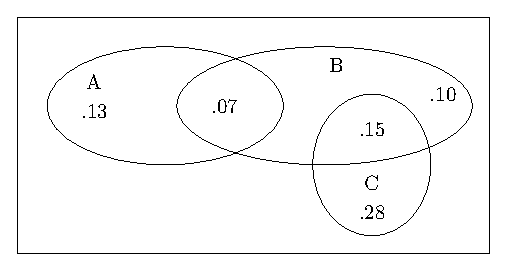
\includegraphics[scale=1]{Figures/new-figure0}


\textbf{Solution.}
\begin{enumerate}[label=(\alph*)]
\item 
Clearly,
\begin{align}
\pr{A} &= 0.13 + 0.07\\
       &= 0.20
\end{align}
\item 
Clearly,
\begin{align}
\label{eq:1}
    \pr{B} &= 0.10 + 0.07 + 0.15\\
       &= 0.32
\end{align}
Also,
\begin{align}
A &= A \brak{B+B^{\prime}} =  AB + AB^{\prime}\\
[&\because B + B^\prime = 1]\\\label{eq:axiom_sum_A}
\pr{A} &= \pr{AB} +\pr{AB^\prime}\\
    [&\because BB^\prime = 0] \nonumber
\end{align}
Using \eqref{eq:axiom_sum_A}
\begin{align}
    \pr{BC^\prime} &= \pr{B} - \pr{BC} \\
    &= 0.32 - 0.15\\
    &= 0.17
\end{align}
\item 
From Axioms of Probability
\begin{align}
\label{Axioms}
    \pr{A + B} &= \pr{A} + \pr{B} - \pr{AB}\\
    &= 0.20 + 0.32 - 0.07\\
    &= 0.45
\end{align}
\item 
Using \eqref{eq:axiom_sum_A}
\begin{align}
    \pr{AB^\prime} &= \pr{A} - \pr{AB} \\
    &= 0.20 - 0.07\\
    &= 0.13
\end{align}
\item 
Clearly,
\begin{align}
    \pr{BC} = 0.15
\end{align}
\item 
Let $X$ be the event that exactly one of $A$, $B$ or $C$ occur.

Let $Y$ be the event that at least one of $A$, $B$ or $C$ occur.

Using Boolean logic,
\begin{align}
    Y=A+B+C
\end{align}
Let $Z$ be the event that at least two of A, B or C occur.

Writing down $Z$ as at least one of $AB$, $BC$ or $AC$ occurring gives us.
\begin{align}
    Z=AB+BC+CA
\end{align}
We know that, all three events never occur simultaneously.

Therefore,

$Z$ represents occurrence of exactly 2 of A,B and C.

$X$ represents occurrence of exactly 1 of A,B and C.

$Y$ can therefore be written as,
\begin{align}
    Y&=X+Z\\
    YZ^\prime&=(X+Z)Z^\prime\\
    YZ^\prime&=XZ^\prime+ZZ^\prime\\
    YZ^\prime&=XZ^\prime
\end{align}
$Z^\prime$ can be thought of as either none of the events occurring or exactly one of them occurring

$XZ^\prime$ would therefore be event that exactly one occurs.
\begin{align}
    XZ^\prime&=X\\
    X&=YZ^\prime\\
    &=(A+B+C){(AB+BC+CA)}^\prime\\
    &=(A+B+C){(AB)}^\prime{(BC)}^\prime{(CA)}^\prime \\
    &=(A+B+C)(A^\prime + B^\prime)(B^\prime + C^\prime)(A^\prime + C^\prime) \\
    &=(AA^\prime+BA^\prime+CA^\prime+AB^\prime+BB^\prime+CB^\prime)\nonumber\\
    &(B^\prime A^\prime+C^\prime A^\prime+B^\prime C^\prime +C^\prime C^\prime)\\
    &=(BA^\prime+CA^\prime+AB^\prime+CB^\prime)(A^\prime B^\prime\nonumber\\
    &+A^\prime C^\prime+B^\prime C^\prime)\\
    &=(BA^\prime A^\prime B^\prime+BA^\prime A^\prime C^\prime+BA^\prime B^\prime C^\prime\nonumber\\
    &+CA^\prime A^\prime B^\prime +BA^\prime A^\prime C^\prime+CA^\prime B^\prime C^\prime\nonumber\\
    &+AB^\prime A^\prime B^\prime+ AB^\prime A^\prime C^\prime+AB^\prime B^\prime C^\prime\nonumber\\
    &+CB^\prime A^\prime B^\prime+ CB^\prime A^\prime C^\prime +CB^\prime B^\prime C^\prime)\nonumber\\
    &=(A^\prime BC^\prime+A^\prime B^\prime C+AB^\prime C^\prime)
\end{align}
Now, $X$ has been represented as a union of 3 mutually exclusive events.

As any 2 of them has 0 intersection due of presence of complements.

Therefore, by Axioms of Probability
\begin{align}
    \pr{X}&=\pr{AB^\prime C^\prime}+\pr{A^\prime BC^\prime}+\pr{A^\prime B^\prime C}
\end{align}
Clearly, from the figure
\begin{align}
    \pr{X}&=0.13+0.10+0.28\\
    &=0.51
\end{align}

\end{enumerate}
\end{document}